% !TEX encoding = UTF-8
% !TEX TS-program = pdflatex
% !TEX root = ../tesi.tex

%**************************************************************
\chapter{Strumenti e tecnologie utilizzate}
\label{cap:strumenti-tecnologie}

%**************************************************************

\intro{Tale capitolo racchiude gli strumenti utilizzati e le tecnologie impiegate durante la realizzazione di \myTitle. In particolare verra analizzato il dominio di utilizzo di esse e le varie meotodologie utilizzate.}\\

%**************************************************************
\section{Apache Flink}
\textit{Apache Flink} è un \gls{framework} di \textit{data processing engine} per l'elaborazione e processamento di dati in modo distribuito.
La forza di Flink è quella di trattare dati in differenti formati, opportuni per il dominio applicativo più consono per l'utente, infatti i dati possono essere di tipo \gls{stateful} che \gls{stateless} e tali flussi possono essere illimitati (\gls{unbounded streams}) o limitati (\gls{bounded streams}). Flink è stato progettato per funzionare in tutti i comuni ambienti \gls{cluster}.

\subsection{DataStream e DataStrem API}
In Apache Flink i dati processati in un programma vengono rappresentati dalla classe speciale \textit{DataStream}.
Tali dati possono essere finiti o illimitati, e le \gls{api} utilizzate per lavorare su questi due differenti tipoligie di dati è la stessa, rendendo il tutto trasparente per l'utente programmatore.\\
Carattestiche fondamentali dei \textit{DataStream} sono:
\begin{itemize}
	\item{\textbf{immutabilità:} una volta creati non è possibile aggiungere o rimuovere elementi;}
	\item{\textbf{soggetti a trasformazioni:} non è possibile ispezionare gli elementi al proprio interno, ma solo lavorare su di essi utilizzando le \textit{DataStream \gls{api}}, che vengono definite, appunto, trasformazioni.}
\end{itemize}
La creazione di un \textit{DataStream} necessità di avere una sorgente iniziale (la quale può essere, per esempio, una coda \gls{kafka}) e da questo si possono derivare numerosi flussi e combinarli utilizzando le \gls{api} esposte, nonchè gli operatori descritti nella sezione \S\ref{sec:operatori}.
Le \textit{DataStream \gls{api}} supportano differenti modalità di esecuzione, le quali permettono di avere un approccio più mirato in base all'utilizzo effettivo dell'utente.\\
Le modalità principali di esecuzione sono:
\begin{itemize}
	\item{\textbf{Esecuzione streaming:} tratta principalmente di flussi illimitati (\gls{unbounded streams}) i quali hanno la caratteristica di non terminare mai. I dati vengono processati ininterrottamente, continuando ad aggiornare l'ouput prodotto. In questa modalità le attività esecutive all'interno della \gls{pipeline} del programma continuano ad essere processate in contemporanea, senza stanziarsi in una fase specifica. Questo implica che la \gls{pipeline} non arriverà mai ad uno stadio di terminazione;}
	\item{\textbf{Esecuzione batch:} tratta solo flussi limitati (\gls{bounded streams}). Questa procedura permette a Flink di ottimizzare l'esecuzione basandosi sul flusso conosciuto, il quale ha un'inizio ed una fine. In questa modalità le varie attività all'interno della \gls{pipeline} del programma possono essere eseguite una dopo l'altra, permettendo di passare alla fase successiva solo quando si è terminata quella precedente (quindi non in contemporanea come avviene per l'esecuzione streaming). I dati fra una fase ed un'altra vengono salvati in una memoria non temporanea per permettere a Flink di ripartire da un determinato step senza rieseguire l'intero programma.}
\end{itemize}

\subsection{Table API}
Apache Flink dispone di due \gls{api} relazionali, l'\textit{\gls{api} Table} e \textit{\gls{sql}}, per un flusso unificato e l'elaborazione batch. L'\gls{api} Table consente la composizione di \gls{query} da operatori relazionali come selezione, filtro e join in modo molto intuitivo. Le \gls{query} specificate in entrambe le interfacce hanno la stessa semantica e specificano lo stesso risultato indipendentemente dal fatto che l'input sia continuo (streaming) o limitato (batch).\\
In particolare l'\textit{\gls{api} Table} è un super set del linguaggio \gls{sql} ed è appositamente progettato per lavorare con Apache Flink. L'\gls{api} Table è un'\gls{api} integrata nel linguaggio per Scala, Java e Python. Invece di specificare le \gls{query} come valori di tipo stringa come nel comune linguaggio \gls{sql}, vengono definite in uno stile integrato nel linguaggio in Java, Scala o Python.

\subsubsection{Query e DataStream}
La tabella sootostante mette a confronto l'algebra relazionale tradizionale e l'elaborazione di un flusso illimitato riguardo i dati in input, l'esecuzione e l'output finale.

\begin{table}[hbt!]
\caption{Tabella di confronto fra l'algebra relazione e l'elaborazione di un flusso illimitato}
\label{tab:algebraRelazionale-flussoIllimitato}
\begin{tabularx}{\textwidth}{XX}
\hline
\textbf{Algebra relazionale} & \textbf{Flusso illimitato}\\
\hline
Le relazioni (o tabelle) sono (multi)insiemi limitati di tuple.     & Un flusso illimitato è una sequenza infinita di tuple. \\
\hline
Una \gls{query} eseguita su dati batch (ad esempio, una tabella in un database relazionale) ha accesso ai dati di input completi.    & Una \gls{query} su un flusso illimitato non può accedere a tutti i dati quando viene eseguita e deve aspettare la trasmissione dei dati. \\
\hline
Una \gls{query} eseguita su dati batch termina dopo aver prodotto un risultato fissato, cioè non modificabile dopo l'esecuzione. & Una \gls{query} su un flusso illimitato aggiorna continuamente il suo risultato in base ai record ricevuti e non viene mai completata. \\
\hline
\end{tabularx}
\end{table}%

Come si evince, i flussi illimitati non lavorano su tabelle statiche, bensì dinamiche. Infatti, le \textit{Dynamic tables} sono il concetto centrale delle Table \gls{api} di Flink per permettere ad esse di lavorare su un flusso streaming.\\
Le tabelle dinamiche cambiano nel tempo e l'interrogazione su di esse produce una \}gls{query continua, ed essa produce risultati dinamici, aggiornando continuamente la sua tabella dei risultati (dinamica) per riflettere le modifiche sulle sue tabelle di input (dinamiche). È importante notare che un output di una \gls{query} continua è sempre semanticamente equivalente al risultato della stessa \gls{query} eseguita in modalità batch su uno \gls{snapshot} delle tabelle di input.



\subsection{Operatori}\label{sec:operatori}
Gli operatori di Flink sono delle procedure per trasformare \textit{DataStream} in altri \textit{DataStream}. Sono utilizzati principalmente per modificare il tipo di flusso di un \textit{DataStream}, il quale appunto verrà filtrato, mappato o combinato con altri flussi per produrre un differente \textit{DataStream}. Nelle sezioni sottostanti verranno descritti i principali operatori utilizzati, i quali non rappresentano la totalità degli operatori disponibili. Per l'elenco completo si rimanda alla documentazione ufficiale di Apache Flink.

\subsubsection{FlatMap}
Operatore che dato un elemento, ne produce in output uno, zero o molteplici. Tale operatore trasformerà un dato \textit{DataStream} in un altro \textit{DataStream}. La procedura di trasformazione è definita dall'utente e per ogni elemento del \textit{DataStream} verrà applicata tale logica per andare a definire l'output atteso. Di seguito la struttura appena descritta.

\begin{minted}{scala}
dataStream.flatMap { str => str.split(" ")}
\end{minted}
	
	
\subsubsection{CoFlatMap}
Operatore che dato un elemento, ne produce in output uno, zero o molteplici. Tale operatore trasforma un \textit{ConnectedStream} in un \textit{DataStream}. La differenza con l'operatore \textbf{FlatMap} è che tale operatore lavorerà su due \textit{DataStream} connessi fra di loro, e come per l'operatore nella sezione precedente, verrà prodotto in output un unico \textit{DataStream} secondo una logica definita dall'utente. Di seguito la struttura appena descritta.

\begin{minted}{scala}
connectedStreams.flatMap(
    (_ : Int) => true,
    (_ : String) => false
)
\end{minted}

\subsubsection{KeyBy}
Operatore che suddivide un flusso in partizione disgiunte. Tale operatore trasforma un \textit{DataStream} in un \textit{KeyedStream} trattando gli elementi che hanno chiave uguale nella stessa partizione. Internamente, \textit{KeyBy} è implementato con il partizionamento hash.
La chiave deve essere intesa come univoca.
Di seguito la struttura appena descritta.
\begin{minted}{scala}
dataStream.keyBy(_.someKey)
dataStream.keyBy(_._1)
\end{minted}

\subsubsection{ProcessFunction}
Operatore di basso livello che da accesso ai blocchi base di uno \textit{Stream}:
\begin{itemize}
	\item{\textbf{eventi:} elementi dello stream;}
	\item{\textbf{stati:} stati tolleranti agli errori, consistenti e supportati solo nei \textit{KeyedStream}. La \textit{ProcessFunction} da accesso allo stato tramite il \textit{RuntimeContext}, in modo simile a quanto avviene negli altri operatori che hanno accesso allo stato;}
	\item{\textbf{timer:} tempo relativo all'evento e tempo relativo al processamento dei dati, anch'esso supportato solo nei \textit{KeyedStream}. Per una descrizione più approfondità del timer farè riferimento alla sezione \S\textbf{Timer} sottostante.}
\end{itemize}

Per creare una \textit{ProcessFunction}, serve implementare il metodo astratto \textit{processElement}, nella quale va implementata la logica di gestione degli elementi. Inoltre, per usufruire dello \textbf{state} e del \textbf{timer}, come descritto precedentemente, bisogna basarsi su un \textit{KeyedStream}. Di seguito è stato deciso di analizzare due principali operatori derivati dalla \textit{ProcessFunction}, quali \textbf{KeyedProcessFunction} e \textbf{KeyedBroadcastProcessFunction}, ampiamente utilizzati durante il perido di stage.

\myParagraph{KeyedProcessFunction}
La \textit{KeyedProcessFunction} è un'estensione di \textit{ProcessFunction}, la quale permette l'accesso alla chiave dei timer nel suo metodo \textbf{onTimer}. Di seguito un esempio relativo all'estensione della classe \textit{KeyedProcessFunction}, dove all'interno del metodo \textit{onTimer} avviene l'accesso alla chiave dei timer. I parametri \textbf{K}, \textbf{I} e \textbf{O} indicano rispettivamente il \textbf{tipo della chiave}, il \textbf{tipo dell'elemento in input} e il \textbf{tipo dell'elemento in output}.

\begin{minted}{scala}
class Example extends KeyedProcessFunction[K, I, O] {

  override def processElement(
      value: I, 
      ctx: KeyedProcessFunction[K, I, O]#Context, 
      out: Collector[O]): Unit = {
      
      	// ...
  }

  override def onTimer(
      timestamp: Long, 
      ctx: KeyedProcessFunction[K, I, O]#OnTimerContext, 
      out: Collector[O]): Unit = {
      
      	var key = ctx.getCurrentKey
      
      	// ...
  }
}
\end{minted}
\myParagraph{KeyedBroadcastProcessFunction}
La \textit{KeyedBroadcastProcessFunction} è un'estensione di \textit{ProcessFunction}, la quale permette l'elaborazione di due flussi entranti, quello \textit{broadcast} e quello \textit{non broadcast}. Il punto chiave di questo operatore è che il \textbf{Broadcast State}, il quale viene gestito dal flusso broadcast, è condiviso fra tutte le istanze parallele dell'operatore, quindi ogni calcolo effettuato in questo flusso garantirà una modifica allo stato di esso che si rifletterà in ogni istanza dell'operatore, a differenza del lato non \textbf{broadcast}. Di seguito un esempio relativo all'estensione della classe \textit{KeyedBroadcastProcessFunction}, dove i parametri \textbf{K}, \textbf{I1}, \textbf{I2} e \textbf{O} indicano rispettivamente il \textbf{tipo della chiave}, il \textbf{tipo dell'elemento in input nel flusso non broadcast}, il \textbf{tipo dell'elemento in input nel flusso broadcast} e il \textbf{tipo dell'elemento in output}.
\begin{minted}{scala}
class Example extends KeyedBroadcastProcessFunction[K, I1, I2, O] {

  override def processElement(
      value: I1, 
      ctx: KeyedBroadcastProcessFunction[K, I1, I2, O]#ReadOnlyContext, 
      out: Collector[O]): Unit = {
      
      	// ...
  }
  
  override def processBroadcastElement(
      value: I2, 
      ctx: KeyedBroadcastProcessFunction[K, I1, I2, O]#Context, 
      out: Collector[O]): Unit = {
      
      	// ...
  }
}
\end{minted}

\myParagraph{Timer}\label{sec:timer}
Tutti e due i tipi di timer (tempo relativo all'evento e tempo relativo processamento di tale) sono gestiti dal \textit{TimeService}. Ogni volta che viene chiamato l'operato \textit{ProcessElement} viene fornito un oggetto chiamato \textit{Context} il quale da accesso al \gls{timestamp} relativo all'evento e ad un oggetto chiamato \textit{TimeService}, il quale permette di registrare il timer per permettere future elaborazioni. Per ogni coppia \textit{chiave}-\gls{timestamp} esiste un solo timer, se più timer sono settati per lo stesso \gls{timestamp}, solo uno verrà richiamato. Flink sincronizza internamente l'invocazione della funzione \textit{processElement} e \textit{onTimer}, rendendo tale sincronizzazione trasparente per l'utente. I timer sono tolleranti verso gli errori, infatti Flink salva tale timer tramite il meccanismo di \gls{checkpoint} come avviene per gli stati.


\subsection{Scalabilità}
Flink è progettato per eseguire applicazioni di streaming \gls{stateful} su qualsiasi scala. Le applicazioni vengono parallelizzate in migliaia di attività che vengono distribuite ed eseguite contemporaneamente in un \gls{cluster}. Pertanto, un'applicazione può sfruttare quantità virtualmente illimitate di CPU, memoria principale, disco e Input-Output di rete. Inoltre, Flink riesce a gestire quantità elevate di stati all'interno dell'applicazione e grazie al suo algoritmo di checkpoint asincrono e incrementale assicura un impatto minimo sulle latenze di elaborazione, garantendo al tempo stesso il processamento dello stato esattamente una ed una sola volta.

\subsection{Alta disponibilità e recovery}
Durante l'elaborazione dei dati in Apache Flink può essere necessario memorizzare le informazioni ricevute ad un dato istante dell'elaborazione, come per esempio quando si addestra un modello di machine learning su un flusso di punti dati, oppure quando è necessario gestire i dati storici. Per fare ciò Flink utilizza il meccanisco di salvataggio delle informazioni in \textbf{stati}.\\
Per gestire tale meccanismo, in Flink vengono sfruttate le chiavi passati durante l'elaborazione di un flusso. Lo stato relativo alla chiave viene mantenuto in quello che può essere considerato un archivio chiave/valore incorporato. Pertanto, l'accesso allo stato chiave/valore è possibile \textbf{solo su flussi con chiave}. L'allineamento delle chiavi dei flussi e dello stato assicura che tutti gli aggiornamenti su di esso siano operazioni locali, garantendo la coerenza senza sovraccarico delle transazioni. Questo allineamento consente inoltre a Flink di ridistribuire lo stato e regolare il partizionamento del flusso in modo trasparente per l'utente programmatore.

\begin{figure}[!h] 
    \centering 
    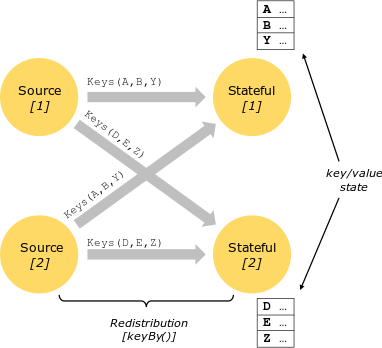
\includegraphics[width=0.5\columnwidth]{tecnologieUtilizzate/flink/state_partitioning.png} 
    \caption{Parallelizzazione del processamento del flusso per chiave in Apache Flink}
\end{figure}

\subsubsection{Checkpoint}
Durante l'elaborazione dei dati possono avvenire degli errori che non permettono la continuità del processamento dei dati. Flink permette di essere tollerante a questi errori tramite il meccanismo di \textbf{checkpoint}. Un checkpoint contrassegna un punto specifico in ciascuno dei flussi di input insieme allo stato corrispondente per ciascuno degli operatori. Un flusso di dati in streaming può essere ripreso da un checkpoint mantenendo la coerenza (cioè elaborando il dato essatamente una volta) ripristinando lo stato degli operatori e riproducendo i record dal punto prefissato dal checkpoint.\\
Durante il processamento, in caso di errori (come errori di rete), Flink interrompe il flusso di dati in streaming ed esegue le seguenti operazionie:
\begin{itemize}
	\item{Il sistema riavvia gli operatori e li reimposta sull'ultimo checkpoint riuscito;}
	\item{I flussi di input vengono reimpostati al dato \gls{snapshot} dello stato.}
\end{itemize}
Inoltre viene garantito che tutti i record elaborati come parte del flusso di dati parallelo riavviato non abbiano influito sullo stato del checkpoint precedente.
Il meccanismo di checkpoint (sia a livello di creazione che di ripristino da esso), se configurato durante l'elaborazione, è totalmente gestito da Flink, rendendolo trasparente per l'utente.

\subsubsection{Savepoint}
Tutti i programmi che utilizzano il checkpoint possono riprendere l'esecuzione da un \textbf{savepoint}. I savepoint  consentono di aggiornare i programmi (quindi la logica al loro interno) che il \gls{cluster} di Flink.\\
I savepoint si possono considerare come dei veri e propri checkpoint, che acquisiscono uno \gls{snapshot} del programma e lo scrivono in un backend di stato. Si affidano al normale meccanismo di checkpoint, descritto precedentemente, per fare ciò. La differenza sostanziale con un checkpoint è che il savepoint:
\begin{itemize}
	\item{vengono creati manualmente dall'utente;}
	\item{non vengono eliminati quando viene eseguito un checkpoint in un dato istante successivo al savepoint.}
\end{itemize}


\subsection{Serializzazione}
Per salvare e ripristinare i dati durante la creazione di un checkpoint o savepoint, Flink serializza e deserializza i dati in formato binario. Questo rende comprensibile il formato dei dati in qualunque sistema di gestione di essi.\\
Flink pone alcune restrizioni sul tipo di elementi che possono trovarsi in un \textit{DataSet} o \textit{DataStream}. La ragione di ciò è che il sistema analizza i tipi per determinare strategie di esecuzione più efficienti. Esistono sette diverse categorie di tipi di dati:
\begin{itemize}
	\item{\textbf{Tuple di Java} e \textbf{Case class di Scala:} Le \textit{Tuple} sono tipi compositi che contengono un numero fisso di campi di diverso tipo. Invece Le Case class di Scala (e le Tuple Scala che sono un caso particolare delle Case class) sono tipi compositi che contengono un numero fisso di campi di tipo diverso;}
	\item{\textbf{Java \gls{POJO}}: Le classi Java e Scala sono trattate da Flink come un tipo di dati POJO speciale se soddisfano i seguenti requisiti:
\begin{itemize}
	\item{la classe deve essere pubblica;}
	\item{deve avere un costruttore pubblico senza argomenti (costruttore predefinito);}
	\item{tutti i campi sono pubblici o devono essere accessibili tramite le funzioni getter e setter;}
	\item{il tipo di un campo deve essere supportato da un serializzatore registrato.}
\end{itemize}}
	\item{\textbf{tipi primitivi:} Flink supporta tutti i tipi primitivi Java e Scala;}
	\item{\textbf{classi generali:} Tutte le classi che non sono identificate come tipi POJO (vedi i requisiti \gls{POJO} sopra) sono gestite da Flink come tipi di \textit{classe generali}. Flink tratta questi tipi di dati come scatole nere e non è in grado di accedere al loro contenuto (ad esempio, per un ordinamento efficiente). I tipi generali vengono de/serializzati utilizzando il framework di serializzazione Kryo.;}
	\item{\textbf{valori};}
	\item{Hadoop Writables;}
	\item{Special Types.}
\end{itemize}

\subsubsection{Avro}

\subsubsection{Kryo}




\section{Scala}

\section{Amazon Kinesis}

